% =====================================================================
% AAMAS 2027 sigconf body. Numbers trace to recomputation from the
% released matrices, the public DevAI release, or the explicitly reported
% replication artifacts in analysis/aamas_2027/results.
% =====================================================================
\documentclass[sigconf,anonymous]{aamas}
\usepackage{array}
\usepackage{tikz}
\usetikzlibrary{arrows.meta}
\definecolor{oiBlue}{RGB}{0,114,178}
\definecolor{oiVermil}{RGB}{213,94,0}
\definecolor{oiGreen}{RGB}{0,158,115}
\definecolor{oiPurple}{RGB}{204,121,167}
\newtheorem{proposition}{Proposition}

% AAMAS-2027 copyright block from the official template (do not change)
\makeatletter
\gdef\@copyrightpermission{
  \begin{minipage}{0.2\columnwidth}
%   \href{https://creativecommons.org/licenses/by/4.0/}{
\includegraphics[width=0.90\textwidth]{by}}
  \end{minipage}\hfill
  \begin{minipage}{0.8\columnwidth}
   \href{https://creativecommons.org/licenses/by/4.0/}{This work is licensed under a Creative Commons Attribution International 4.0 License.}
  \end{minipage}
  \vspace{5pt}
}
\makeatother

\setcopyright{ifaamas}
\acmConference[AAMAS 2027]{Proc.\@ of the 26th International Conference
on Autonomous Agents and Multiagent Systems (AAMAS 2027)}{3--7 May 2027}{Hanoi, Vietnam}{M.~Baldoni, F.~Fang, W.~Yeoh, N.~Yorke-Smith (eds.)}
\copyrightyear{2027}
\acmYear{2027}
\acmDOI{}
\acmISBN{}
% Printed on page 1 in anonymous mode. OpenReview submission 1655.
% The official aamas.cls defines \submissionType;
% an undefined-command error indicates a missing or mismatched class file.
\acmSubmissionID{1655}
\submissionType{Research Paper Track}

\title[Language-Conditioned Rank Reversal in LLM Judges]{Language-Conditioned Rank Reversal in Agentic LLM Judges}
\author{Anonymous Author}
\affiliation{%
  \institution{Anonymous Institution}
  \city{Anonymous City}
  \country{United Kingdom}}
\email{anonymous@example.com}

\begin{abstract}
An agentic code evaluator scores an agent's work against written
requirements. Its score can change when the requirements and judging
instructions are localized, even if the code is identical. We study this
effect on a balanced multilingual panel and show that evaluator severity
can reverse across languages. We model the score as task, language,
evaluator, and language-by-evaluator components. The last component is
identified by double centering the score matrix, without human labels.
We state when that estimate is unbiased and give a task-level uncertainty
bound. On held-out tasks, removing the interaction makes evaluator rankings
and quality-gate decisions more consistent across languages. A separate
preference benchmark shows a similar ranking pattern. Consistency is not
accuracy: the correction leaves a language's evaluator-panel mean
unchanged, and this study does not establish a gain in judging correctness
against the code-benchmark labels.
\end{abstract}
\keywords{Agent-as-a-Judge, multilingual evaluation, LLM evaluation, calibration, language bias}
\begin{CCSXML}
<ccs2012>
 <concept>
  <concept_id>10010147.10010178.10010179</concept_id>
  <concept_desc>Computing methodologies~Natural language processing</concept_desc>
  <concept_significance>500</concept_significance>
 </concept>
 <concept>
  <concept_id>10010147.10010178.10010219.10010220</concept_id>
  <concept_desc>Computing methodologies~Multi-agent systems</concept_desc>
  <concept_significance>500</concept_significance>
 </concept>
 <concept>
  <concept_id>10002944.10011122.10002945</concept_id>
  <concept_desc>General and reference~Evaluation</concept_desc>
  <concept_significance>300</concept_significance>
 </concept>
</ccs2012>
\end{CCSXML}
\ccsdesc[500]{Computing methodologies~Natural language processing}
\ccsdesc[500]{Computing methodologies~Multi-agent systems}
\ccsdesc[300]{General and reference~Evaluation}

\begin{document}
\maketitle

%=====================================================================
\section{Introduction}

Agentic systems increasingly use language models to assess other agents.
Agent-as-a-Judge pipelines compare an agent's artifacts with written
requirements \citep{zhuge2024agentjudge}. Their scores
can decide whether a task passes a quality gate. If the score changes with
the language of the rubric, the same artifact may receive a different
decision.

Multilingual judge studies report inconsistent scores and preferences
\citep{hada-etal-2024-large,fu2025reliable,yin2026judgels}. In many studies,
changing the language also changes the response being judged. A score
difference may then come from the judge or from the translated response.
Section~\ref{sec:attribution} explains why scores
alone cannot separate these explanations. Judge-panel averaging and
psychometric audits \citep{zhu2026cyclicjudge,usami2026darkcurrent}
address other sources of evaluator variation. Our target is an offset
that varies jointly with language and evaluator.

We hold the code artifact fixed and vary the localized judging inputs:
requirements, rubric, and judge instructions. This design attributes the
observed score differences to the judging setup rather than to changed code.
It does not separate the model's behavior from differences introduced when
the requirements are translated. We estimate both a shift shared across
evaluators and an interaction between language and evaluator. We then ask
whether that interaction changes quality-gate decisions and whether it is
larger than variation between repeat judge calls.

We study whether evaluator severity reverses across languages, how to
estimate the language-by-evaluator interaction, and what removing it does
to both evaluator rankings and task-level decisions. We combine a fixed-code
audit, formal properties of double centering, held-out analyses on two
benchmarks, and a repeat-call study. We also examine what the
available human labels can and cannot establish about correctness.
Figure~\ref{fig:overview} summarizes the study design and analysis.

\begin{figure*}[t]
\centering
% Figure: study overview. Every number is reported in the body:
% GPT-4o minus GPT-5.4 gap (Table rev), the GPT-4o Spanish cell (Sec. 5.1),
% held-out Kendall tau (Table ranking), held-out gate-25 reduction (Sec. 5.4).
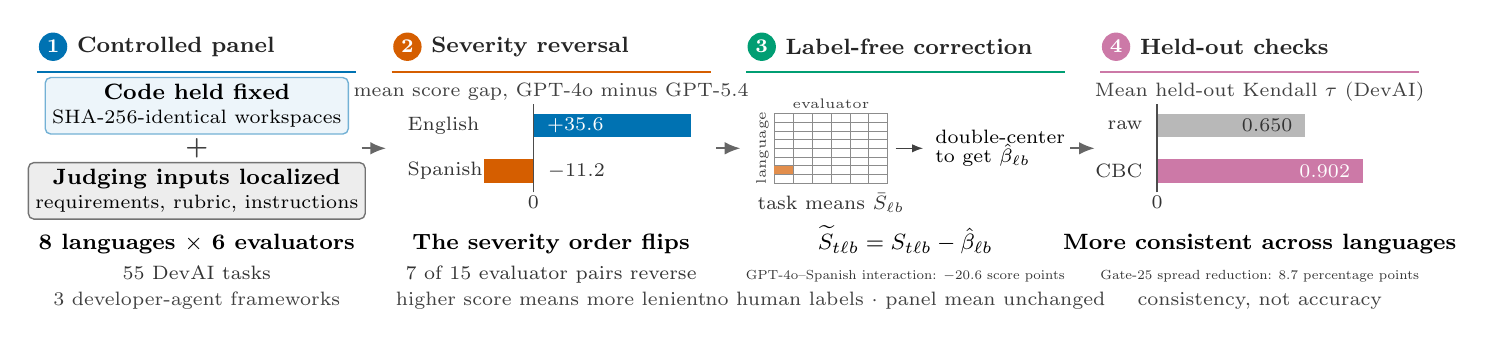
\begin{tikzpicture}[
  x=1cm, y=1cm, font=\footnotesize,
  num/.style={circle, fill=#1, text=white, font=\scriptsize\bfseries,
              inner sep=0pt, minimum size=3.6mm},
  ttl/.style={font=\footnotesize\bfseries, anchor=west, text=black!85},
  card/.style={draw=#1!55, fill=#1!7, rounded corners=2pt, line width=0.5pt,
               align=center, inner sep=2.5pt, minimum width=3.55cm},
  note/.style={font=\scriptsize, text=black!75, align=center},
  flow/.style={-{Latex[length=2mm,width=1.6mm]}, line width=0.8pt, draw=black!60},
  bar/.style={draw=none, fill=#1},
  lab/.style={font=\scriptsize, text=black!80},
]
\def\pw{4.05}
\def\pg{0.45}
% Shared baselines keep diagrams and explanatory rows aligned across panels.
\def\ovGraphTop{2.60}
\def\ovGraphBottom{1.72}
\def\ovGraphCenter{2.16}
\def\ovResultY{0.88}
\def\ovDetailY{0.50}
\def\ovFooterY{0.16}

% Panel frame: number badge, title, colored rule.
\newcommand{\ovpanel}[4]{%
  \node[num=#4] at ({#1+0.2},3.45) {#2};
  \node[ttl] at ({#1+0.38},3.45) {#3};
  \draw[#4, line width=1pt] (#1,3.13) -- ({#1+\pw},3.13);
}

\pgfmathsetmacro{\xa}{0}
\pgfmathsetmacro{\xb}{\pw+\pg}
\pgfmathsetmacro{\xc}{2*(\pw+\pg)}
\pgfmathsetmacro{\xd}{3*(\pw+\pg)}

\ovpanel{\xa}{1}{Controlled panel}{oiBlue}
\ovpanel{\xb}{2}{Severity reversal}{oiVermil}
\ovpanel{\xc}{3}{Label-free correction}{oiGreen}
\ovpanel{\xd}{4}{Held-out checks}{oiPurple}

\foreach \s/\e in {\xa/\xb, \xb/\xc, \xc/\xd}
  \draw[flow] ({\s+\pw+0.07},\ovGraphCenter) -- ({\e-0.07},\ovGraphCenter);

% ---------------- 1. controlled panel ----------------
\begin{scope}[shift={(\xa,0)}]
  \node[card=oiBlue] at (\pw/2,2.70)
    {\textbf{Code held fixed}\\[-1pt]{\scriptsize SHA-256-identical workspaces}};
  \node[font=\small\bfseries, text=black!75] at (\pw/2,\ovGraphCenter) {+};
  \node[card=black] at (\pw/2,1.62)
    {\textbf{Judging inputs localized}\\[-1pt]{\scriptsize requirements, rubric, instructions}};
  \node[anchor=base] at (\pw/2,\ovResultY) {\textbf{8 languages $\times$ 6 evaluators}};
  \node[lab, anchor=base] at (\pw/2,\ovDetailY) {55 DevAI tasks};
  \node[note, anchor=base] at (\pw/2,\ovFooterY) {3 developer-agent frameworks};
\end{scope}

% ---------------- 2. severity reversal ----------------
\begin{scope}[shift={(\xb,0)}]
  \pgfmathsetmacro{\zx}{1.8}       % zero line
  \pgfmathsetmacro{\u}{2.0/35.6}   % cm per score point
  \node[note] at (\pw/2,2.88) {mean score gap, GPT-4o minus GPT-5.4};
  \fill[oiBlue]    (\zx,2.30) rectangle ({\zx+35.6*\u},2.60);
  \fill[oiVermil]  ({\zx-11.2*\u},1.72) rectangle (\zx,2.02);
  \draw[black!70, line width=0.5pt] (\zx,1.60) -- (\zx,2.72);
  \node[lab] at (\zx,1.47) {$0$};
  \node[lab, anchor=west] at (0.08,2.45) {English};
  \node[lab, anchor=west, text=white, font=\scriptsize\bfseries] at ({\zx+0.05},2.45) {$+35.6$};
  \node[lab, anchor=west] at (0.08,1.87) {Spanish};
  \node[lab, anchor=west] at ({\zx+0.06},1.87) {$-11.2$};
  \node[anchor=base] at (\pw/2,\ovResultY) {\textbf{The severity order flips}};
  \node[lab, anchor=base] at (\pw/2,\ovDetailY) {7 of 15 evaluator pairs reverse};
  \node[note, anchor=base] at (\pw/2,\ovFooterY) {higher score means more lenient};
\end{scope}

% ---------------- 3. label-free correction ----------------
\begin{scope}[shift={(\xc,0)}]
  \def\cw{0.24}
  \pgfmathsetmacro{\ch}{(\ovGraphTop-\ovGraphBottom)/8}
  \pgfmathsetmacro{\gx}{0.36}
  \pgfmathsetmacro{\gy}{\ovGraphBottom}
  \foreach \r in {0,...,7}
    \foreach \c in {0,...,5}
      \draw[black!45, line width=0.3pt, fill=white]
        ({\gx+\c*\cw},{\gy+\r*\ch}) rectangle ++(\cw,\ch);
  % GPT-4o column, Spanish row
  \fill[oiVermil!70] ({\gx},{\gy+1*\ch}) rectangle ++(\cw,\ch);
  \node[font=\tiny, text=black!75, rotate=90] at ({\gx-0.15},{\gy+4*\ch}) {language};
  \node[font=\tiny, text=black!75] at ({\gx+3*\cw},{\ovGraphTop+0.13}) {evaluator};
  \node[lab] at ({\gx+3*\cw},1.47) {task means $\bar S_{\ell b}$};
  \draw[-{Latex[length=1.4mm]}, black!75, line width=0.5pt]
    ({\gx+6*\cw+0.1},{\gy+4*\ch}) -- ++(0.35,0);
  \node[align=left, anchor=west, font=\scriptsize] at ({\gx+6*\cw+0.48},{\gy+4*\ch})
    {double-center\\[-1pt]to get $\hat\beta_{\ell b}$};
  \node[anchor=base] at (\pw/2,\ovResultY)
    {$\widetilde S_{t\ell b}=S_{t\ell b}-\hat\beta_{\ell b}$};
  \node[lab, align=center, anchor=base] at (\pw/2,\ovDetailY)
    {\resizebox{\pw cm}{!}{GPT-4o--Spanish interaction: $-20.6$ score points}};
  \node[note, anchor=base] at (\pw/2,\ovFooterY) {no human labels $\cdot$ panel mean unchanged};
\end{scope}

% ---------------- 4. held-out checks ----------------
\begin{scope}[shift={(\xd,0)}]
  \pgfmathsetmacro{\zx}{0.72}
  \pgfmathsetmacro{\u}{2.9}        % cm per unit tau
  \node[note] at (\pw/2,2.88) {Mean held-out Kendall $\tau$ (DevAI)};
  \fill[black!28]  (\zx,2.30) rectangle ({\zx+0.650*\u},2.60);
  \fill[oiPurple]  (\zx,1.72) rectangle ({\zx+0.902*\u},2.02);
  \draw[black!70, line width=0.5pt] (\zx,1.60) -- (\zx,2.72);
  \node[lab] at (\zx,1.47) {$0$};
  \node[lab, anchor=east] at ({\zx-0.06},2.45) {raw};
  \node[lab, anchor=east] at ({\zx-0.06},1.87) {CBC};
  \node[lab, anchor=east] at ({\zx+0.650*\u-0.04},2.45) {$0.650$};
  \node[lab, anchor=east, text=white, font=\scriptsize\bfseries]
    at ({\zx+0.902*\u-0.04},1.87) {$0.902$};
  \node[anchor=base] at (\pw/2,\ovResultY) {\textbf{More consistent across languages}};
  \node[lab, align=center, anchor=base] at (\pw/2,\ovDetailY)
    {\resizebox{\pw cm}{!}{Gate-25 spread reduction: 8.7 percentage points}};
  \node[note, anchor=base] at (\pw/2,\ovFooterY) {consistency, not accuracy};
\end{scope}
\end{tikzpicture}

\caption{Study overview. (1)~Code is held fixed while the judging inputs
are localized. (2)~GPT-4o scores above GPT-5.4 in English and below it in
Spanish (Table~\ref{tab:rev}). (3)~CBC double-centers the task-mean score matrix to
estimate and remove the language-by-evaluator interaction. (4)~On held-out
tasks, severity rankings and gates agree more across languages
(Table~\ref{tab:ranking}, Sec.~\ref{sec:results}); this is consistency,
not accuracy. The grid is schematic.}
\Description{Four stages. First, fixed code with localized judging inputs
over eight languages and six evaluators. Second, a bar chart of the GPT-4o
minus GPT-5.4 mean score gap: plus 35.6 in English and minus 11.2 in
Spanish. Third, the task-mean language-by-evaluator score matrix is
double-centered and the estimated interaction is subtracted from each score;
the GPT-4o Spanish interaction is minus 20.6 score points. Fourth, mean
held-out cross-language Kendall tau rises from 0.650 to 0.902 and gate-25
spread falls by 8.7 percentage points. Higher scores
indicate leniency, not quality.}
\label{fig:overview}
\end{figure*}

\section{Related Work}
\label{sec:related}

\paragraph{LLM-judge reliability.}
\citet{zheng2023judging} document position, verbosity, and self-enhancement
biases when LLMs judge conversational responses. Across twenty NLP tasks,
\citet{bavaresco2025llms} find that agreement with human judgments varies
with the model, task, and property being evaluated. Ratings can also vary
between calls within one language \citep{stureborg2024inconsistent}.
Psychometric audits measure how prompts change decision criteria and
sensitivity to controlled quality changes \citep{usami2026darkcurrent}.
These findings motivate testing both systematic language effects and
repeat-call variation, rather than treating every score difference as a
stable evaluator characteristic.

\paragraph{Multilingual evaluation.}
\citet{hada-etal-2024-large} compare multilingual ratings with native-speaker
judgments and find score inflation. Other studies report differences in
judge agreement across languages \citep{fu2025reliable,babeljudge2026}.
MM-Eval assesses multilingual judging through both pairwise decisions and
the consistency and fairness of absolute scores \citep{son2024mmeval}.
The CIA suite combines a human-annotated multilingual test set with Hercule,
an evaluator that uses English reference answers to score responses in
other languages \citep{doddapaneni2025cross}.
\citet{sheth2026crosslingual} decompose evaluations into shared criteria
and learn a transfer module from English labels, without target-language
annotations. These approaches evaluate or adapt multilingual judges;
we estimate interactions from an already collected score panel.
\citet{yin2026judgels} test preference stability under English, Chinese,
and mixed-language presentations of response pairs, including translated
responses. Our fixed-code design instead changes the judging inputs and
measures quality-gate consequences. It still mixes judge behavior with
translation of the requirements.

\paragraph{Calibration and aggregation.}
CalibraEval uses label-free distribution correction to reduce selection
bias when response positions or option identifiers change
\citep{li2025calibraeval}. Dawid--Skene estimates observer error rates for
categorical labels when the true labels are unavailable
\citep{dawid1979maximum}. Such latent-label estimation has a different
target from decomposing absolute score means.
Judge-aware pairwise models estimate evaluator-specific discrimination
\citep{xu2026judgeaware}, while heterogeneous judge-aware ranking models
consensus and structured disagreement \citep{yu2026heterogeneous}.
Round-robin assignment can recover a benchmark's judge-panel mean at a
single-judge budget \citep{zhu2026cyclicjudge}.
Labeled calibration uses signals from a diverse judge panel
\citep{li2026calibrate}; human anchors are needed to test accuracy
\citep{lee2026report}. Our CBC applies standard two-way ANOVA double
centering \citep{scheffe1959analysis,searle1971linear} to a
language-by-evaluator interaction. It requires a balanced panel for the
stated identification result and leaves the shared language shift intact.

\paragraph{Agentic code judging.}
Agent-as-a-Judge supplies requirement-level evaluation of agent-produced
artifacts and the DevAI benchmark \citep{zhuge2024agentjudge}. The earlier
five-language localization study finds language and backbone sensitivity
in this setting \citep{mahmood2026multilingualpromptlocalizationagentasajudge}.
Automated validation of software-artifact evaluators provides a complementary
way to test a judge \citep{fandina2025refine}.
We audit byte-identical code across localized judging conditions and study
whether interaction correction stabilizes evaluator severity rankings and
quality gates. A separate M-RewardBench preference panel
\citep{gureja-etal-2025-rewardbench} checks ranking consistency on a different
benchmark subset and collection protocol. Neither check establishes that
the corrected code judgments are more accurate.

%=====================================================================
\section{Score Model and Fixed Artifacts}
\label{sec:attribution}

Let $t$, $\ell$, and $b$ index tasks, languages, and evaluator backbones.
Let $n$, $k$, and $m$ be their respective counts.
The score is the mean across the three balanced developer-agent framework
arms for that cell. We use the following additive model:
\begin{equation}
S(t,\ell,b) = \mu(t)+\alpha(b)+g(\ell)+\beta(\ell,b)
             +\gamma(t,\ell)+\epsilon(t,\ell,b),
\label{eq:model}
\end{equation}
where $\mu$ is a task effect, $\alpha$ an evaluator offset (severity), $g$ a
language shift shared by evaluators, $\beta$ the
language-by-evaluator interaction, and $\gamma$ a task-language shift
shared by evaluators. We normalize $\beta$ to have zero row and column
sums and $\gamma$ to have zero task mean in each language.
For the theoretical results, we assume
$\mathbb E[\epsilon(t,\ell,b)]=0$ in every cell. Framework effects that do not interact with both language and
evaluator cancel under double centering in this balanced panel. Task-specific
language-by-evaluator deviations enter $\epsilon$; the original panel
cannot separate them from repeat-call noise. Thus $\beta$ is the
task-average interaction for this panel.
These terms describe scores, not judging accuracy.

If the evaluated response is also translated, the same score table can
arise from a language-invariant evaluator seeing different responses or a
language-sensitive evaluator seeing equivalent responses. We avoid that
particular ambiguity by judging the same code. An audit of the six
evaluator packs, three framework directories, and their workspace trees
found the same 4{,}878-file SHA-256 manifest in all eight conditions.
The localized rubric and requirements may still differ in meaning, so
$\beta$ describes the judging setup as a whole.

%=====================================================================
\section{A Fixed-Artifact Panel}
\label{sec:setup}

We extend the earlier five-language Agent-as-a-Judge setting
\citep{mahmood2026multilingualpromptlocalizationagentasajudge} with
Japanese, Spanish, and Swahili. The panel has 7{,}920 judge runs over 6
evaluators, 8
languages, 3 developer-agent frameworks, and 55 DevAI tasks
\citep{zhuge2024agentjudge}, a complete balanced panel of $55\times8\times6$ task-level cells, each
the mean of three framework runs.
The languages are English, Arabic, Turkish, Chinese, Hindi, Japanese,
Spanish, and Swahili. The framework arms are MetaGPT, GPT-Pilot, and OpenHands. The six
evaluator backbones are GPT-4o, GPT-5.4, Claude Sonnet 4.6,
Gemini 3 Flash Preview, DeepSeek-V3.2, and Qwen3.5-9B.
Figures~\ref{fig:heat} and~\ref{fig:gate} shorten Claude Sonnet 4.6
to ``Sonnet 4.6'' and Gemini 3 Flash Preview to ``Gemini 3 Flash'' to fit
their axes. The rerun logs record exact provider-qualified routes;
the original panel did not preserve model snapshot dates.
For the replication reruns, we record the model route, temperature, top-$p$,
workflow, and manifest seed (the seed is not passed to the provider) in the
accompanying JSONL logs. The judge uses
the released parser: a response containing \texttt{<SATISFIED>} is satisfied,
and every other response, including an empty or failed response, is
unsatisfied. The task score is $100$ times the unweighted fraction of
requirements marked satisfied; recorded prerequisites are not used in that
aggregate. A task passes a gate if the score strictly exceeds the threshold.
Requirement text and user queries were translated from English by GPT-4o under a
token-preservation instruction (paths, identifiers, and backtick spans held
fixed); judge templates were localized while keeping the English
\texttt{<SATISFIED>}/\texttt{<UNSATISFIED>} tags. Native speakers with
graduate-level training reviewed the translations for fluency and technical
fidelity, following the protocol of the five-language setting
\citep{mahmood2026multilingualpromptlocalizationagentasajudge}. Localized
system prompts additionally have mean {LaBSE} cosine similarity $0.90$ with
English (range $0.83$--$0.95$ over 35 prompt--language pairs)
\citep{feng2022labse}. A structural audit of the 55-instance MetaGPT pack
finds no requirement-count mismatches, backtick-span mismatches in 14 of 385
non-English instances, and complete tag preservation in every judge prompt. The released original-panel artifacts do not preserve provider
snapshot dates, base URLs, or per-call retry logs; we therefore reproduce
those results from the saved score matrices rather than claim a full
provider-level regeneration.

Evaluators are not on a common scale: mean satisfaction awarded runs from
42.9 (Gemini 3 Flash Preview) to 3.6 (Qwen3.5-9B), and Qwen3.5-9B
awards zero on 82.0\% of cells.
These means order evaluator \emph{leniency}, not evaluator quality.

\subsection{Consensus-based calibration}
Let $\bar S_{\ell b}$ be the task mean, with a dot denoting an average
over that index. We estimate the interaction and adjust scores by
\begin{equation}
\hat\beta_{\ell b}=\bar S_{\ell b}-\bar S_{\cdot b}
-\bar S_{\ell\cdot}+\bar S_{\cdot\cdot},
\qquad
\widetilde S_{t\ell b}=S_{t\ell b}-\hat\beta_{\ell b}.
\label{eq:cbc}
\end{equation}
We call this consensus-based calibration (CBC). Double centering is a
standard two-way ANOVA operation, not a new estimator
\citep{scheffe1959analysis,searle1971linear}. Its target is relative to
the evaluator pool and benchmark. Adjusted scores are not clipped to
$[0,100]$; clipping would break panel-mean invariance.

\begin{proposition}[Identification and panel-mean invariance]
\label{prop:identify}
In a complete balanced panel under Eq.~\ref{eq:model},
$\mathbb E[\hat\beta_{\ell b}]=\beta_{\ell b}$ for any
task-language effect $\gamma(t,\ell)$ shared by evaluators. Moreover,
$m^{-1}\sum_b\widetilde S_{t\ell b}
=m^{-1}\sum_b S(t,\ell,b)$ for every task and language.
\end{proposition}
\noindent\emph{Proof.} The four terms of Eq.~\ref{eq:cbc} cancel
$\mu,\alpha,g,\gamma$ and leave the normalized $\beta$ plus mean-zero
error. The row sum of $\hat\beta$ is zero by construction, proving the
second identity.\hfill$\square$

The identity means CBC cannot change a decision based on the mean score
of all evaluators for one item. It can change an individual evaluator's
decision or the order of evaluator severity. It leaves the shift $g$
shared by evaluators untouched.

\begin{proposition}[Task-level uncertainty]
\label{prop:bound}
Assume $k,m\geq2$, tasks are independent, scores lie in $[0,100]$, and the
double-centered task error has mean zero. Dependence across languages
and evaluators within a task is allowed. With
$c=(1-1/k)(1-1/m)$, for every $x>0$,
\[
\Pr\!\left\{|\hat\beta_{\ell b}-\beta_{\ell b}|\geq x\right\}
\leq 2\exp\!\left(-\frac{n x^2}{80000c^2}\right).
\]
For all $mk$ cells at once, multiply the right side by $mk$.
\end{proposition}
\noindent\emph{Proof.} Double centering one task gives a linear
combination whose positive coefficients sum to $2c$, as do the
absolute negative coefficients. It lies in $[-200c,200c]$.
Hoeffding's inequality across independent tasks and a union bound
give the result.\hfill$\square$

This bound is deliberately conservative. A Gaussian bound with independent
language-evaluator cell noise would be tighter, but
the same artifact is judged in every condition, making that assumption
implausible. We therefore use a task bootstrap for empirical intervals.
For fixed $k$ and $m$, the bound also shows that the estimated interaction
converges to its model target as the number of independent tasks grows.
For gate analyses, we fit $\hat\beta$ on 1{,}000 bootstrap samples and
evaluate on omitted tasks from the same observed language set.

For two evaluators $i,j$, their language-specific mean score gap is
\begin{equation}
d_{ij}(\ell)=\bar S_{\ell i}-\bar S_{\ell j}
=\alpha_i-\alpha_j+\beta_{\ell i}-\beta_{\ell j}
  +\bar\epsilon_{\ell i}-\bar\epsilon_{\ell j}.
\label{eq:gap}
\end{equation}
The task, shared-language, and task-language terms cancel. We call a
pair a \emph{severity reversal} when observed gaps have opposite signs
in two languages. This rules out one observed ordering of severity
that fits every language. It does not rank evaluator quality: higher
scores can simply mean greater leniency.

%=====================================================================
\section{Results}
\label{sec:results}

Rubric language changes which evaluator marks more severely. We first test
that result, then examine its effect on threshold decisions.

\subsection{Language reverses which evaluator is more severe}

Seven of fifteen evaluator pairs reverse their average severity order
across languages (Table~\ref{tab:rev}). The table's witness languages are selected from 28
possible pairs and are descriptive, so we test the total reversal count.
We fit an additive task, language, and evaluator null, permute its residuals
over languages independently within each (task, evaluator) group,
and add the fitted values back on 1{,}000 draws. This diagnostic assumes
residual exchangeability across languages, a stronger condition than
Proposition~\ref{prop:bound}. The
null has a median of one reversal and a maximum of three, against seven
observed (permutation $p=0.001$). Figure~\ref{fig:heat} shows the interaction:
GPT-4o is $-20.6$ points in Spanish and $+11.8$ in English, relative to its
own mean and the shared language effect. Pointwise 95\% bootstrap intervals exclude zero
for 34 of 48 cells. The permutation test applies to the total reversal
count, not to each selected witness pair. The cell intervals are not
multiplicity-adjusted; gate analyses are exploratory.

\begin{table}[t]\centering\small
\setlength{\tabcolsep}{3pt}
\caption{Seven evaluator pairs reverse severity order. Gaps are mean
score differences for the first evaluator.}
\label{tab:rev}
\begin{tabular*}{\columnwidth}{@{\extracolsep{\fill}}lrr@{}}
\toprule
\textbf{Pair} & \multicolumn{2}{c}{\textbf{Gaps (pts)}}\\
\midrule
GPT-4o vs.\ GPT-5.4 & En $+35.6$ & Es $-11.2$\\
GPT-4o vs.\ Gemini 3 Flash Preview & En $+9.5$ & Es $-32.8$\\
GPT-4o vs.\ Claude Sonnet 4.6 & Hi $+30.7$ & Es $-7.2$\\
GPT-4o vs.\ DeepSeek-V3.2 & En $+32.4$ & Es $-4.3$\\
GPT-5.4 vs.\ Claude Sonnet 4.6 & Ja $-9.0$ & Sw $+10.7$\\
GPT-5.4 vs.\ DeepSeek-V3.2 & Zh $-5.0$ & Sw $+14.3$\\
Claude Sonnet 4.6 vs.\ DeepSeek-V3.2 & Ar $+8.5$ & Hi $-4.5$\\
\bottomrule
\end{tabular*}
\par\smallskip\parbox{\columnwidth}{\footnotesize En = English; Es = Spanish;
Hi = Hindi; Ja = Japanese; Sw = Swahili; Zh = Chinese; Ar = Arabic; Tr = Turkish.
Each row uses its most opposed language gaps.}
\end{table}

\begin{figure}[t]\centering
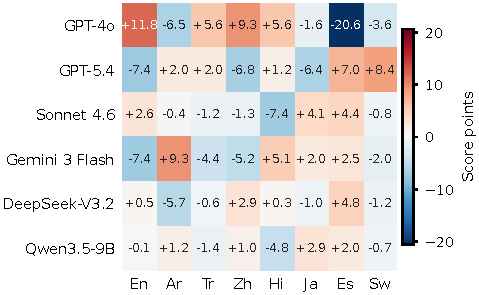
\includegraphics[width=\columnwidth]{figures/fig2_interaction.pdf}
\caption{Centered language-by-evaluator interaction (score points) on
fixed code. Positive values mean higher scores. Language abbreviations
are defined under Table~\ref{tab:rev}; evaluator short labels are
defined in \S\ref{sec:setup}.}
\Description{A six-by-eight heatmap shows the centered score interaction
for each evaluator and language.}
\label{fig:heat}\end{figure}

\subsection{Held-out ranking consistency}
\label{sec:ranking}
We evaluate CBC on tasks omitted from each of 1{,}000 bootstrap fitting
samples, while all eight languages remain observed. The metric is mean
pairwise Kendall $\tau$ between language-specific evaluator
\emph{severity} rankings, over all 28 language pairs. On DevAI, it rises
from $0.650$ to $0.902$ (Table~\ref{tab:ranking}). A language-wide
empirical-Bayes location/scale adjustment adapted from ComBat
\citep{johnson2007combat} gives nearly the same agreement as raw scoring
(equal after rounding to three decimals); it does not estimate the
language-by-evaluator interaction. Quantile normalization
\citep{bolstad2003comparison} performs worse. The paired CBC minus
ComBat difference is positive in all 1{,}000 bootstrap replicates.
These rankings measure which evaluator awards higher scores, not which
one judges code more accurately.

On a separate M-RewardBench preference panel
\citep{gureja-etal-2025-rewardbench}, we collected pointwise 1--5 scores
for the chosen and rejected response of the first 1{,}500 dataset IDs
(805 \texttt{alpacaeval-easy}, 695 \texttt{alpacaeval-hard}), aligned across
English, Arabic, Turkish, Chinese, Hindi, Japanese, and Spanish,
using GPT-4o, GPT-5.4, Claude Sonnet 4.6,
Gemini 3 Flash Preview, and DeepSeek-V3.2. The resulting
10{,}500 language-item instances define 105{,}000 pointwise scores.
Thirty-five of the 52{,}500 evaluator-item-language margins are missing
from the saved score table; the analysis averages available margins
within each cell, excluding missing scores from weighted denominators.
CBC acts on chosen-minus-rejected score margins, which measure preference
strength rather than evaluator severity. Under the same
bootstrap fit and omitted-item evaluation, mean cross-language $\tau$
rises from $0.430$ to $0.900$ (Table~\ref{tab:ranking}). An adapted
judge-aware Bradley--Terry--Luce comparator
\citep{xu2026judgeaware} obtains $0.405$; it uses pairwise evaluator
wins estimated on omitted-item comparisons, excluding pairs with missing
margins, whereas CBC fits continuous-margin interactions on in-bag items.
This is an adapted ranking comparator, not a like-for-like calibration model.
The instance source and
score-collection protocol differ from DevAI, so this result shows
ranking consistency on another panel, not fixed-code attribution.

\begin{table}[t]\centering\small
\setlength{\tabcolsep}{3pt}
\caption{Held-out cross-language ranking agreement. Values are mean
Kendall $\tau$ with 95\% percentile bootstrap intervals.
Bold marks the highest mean per panel.}
\label{tab:ranking}
\begin{tabular*}{\columnwidth}{@{\extracolsep{\fill}}llcc@{}}\toprule
\textbf{Panel} & \textbf{Method} & $\boldsymbol{\tau}$ & \textbf{95\% interval}\\\midrule
DevAI & Raw & 0.650 & [0.610, 0.714]\\
 & Adapted ComBat & 0.650 & [0.610, 0.714]\\
 & Quantile & $-0.097$ & [$-0.119,-0.068$]\\
 & CBC & \textbf{0.902} & [0.795, 0.968]\\\midrule
M-RewardBench & Raw & 0.430 & [0.371, 0.486]\\
 & Adapted BTL & 0.405 & [0.352, 0.467]\\
 & CBC & \textbf{0.900} & [0.790, 1.000]\\
\bottomrule\end{tabular*}
\end{table}

On the full fitting panels, CBC yields $\tau=1$ by construction:
the corrected evaluator means differ between languages only by a shared
additive shift, so their severity or preference-strength rankings coincide.
The omitted-item results in
Table~\ref{tab:ranking} are the relevant stability checks.
A leave-one-language-out DevAI diagnostic rises only from $0.649$ to
$0.740$ when the unseen language receives zero estimated interaction.
It does not establish transfer to unseen languages.

\subsection{Model checks and ablations}
We fit Eq.~\ref{eq:model} to all 7{,}920 framework-level observations
with framework fixed effects. A simplified version without
$\gamma(t,\ell)$ has $R^2=0.691$; including task-language terms gives
$R^2=0.705$. The small $0.015$ increase supports using a compact
description of the panel, but the remaining unexplained variation
warns against treating the interaction as a complete causal account.

Table~\ref{tab:ablations} shows two checks from the DevAI data.
Each evaluator subset uses 100 bootstrap replicates. Subsampling the
evaluator pool leaves mean held-out $\tau$ near $0.90$,
but two-evaluator subsets vary much more than larger subsets. A
separate 100-replicate task-count experiment selects $n$ tasks without
replacement, bootstraps within that subset, and evaluates omitted tasks.
It shows the estimate
approaching the full-panel interaction as the number of tasks grows.
The mean absolute difference falls from 2.01 points with 10 tasks to
0.67 with 55 tasks (Table~\ref{tab:ablations}); the full-panel interaction
is a reference estimate, not ground truth. The $n=55$
value in that experiment differs slightly from the 1,000-replicate
headline because the two loops use independent seeds and protocols.
Splitting requirements by type also gives a larger consistency gain
for model-construction and evaluation-metric checks ($0.737$ to $0.840$)
than for data-loading and training checks ($0.770$ to $0.789$).
These are descriptive ablations, not evidence
that semantic requirements have a uniquely causal language effect.

\begin{table}[t]\centering\small
\setlength{\tabcolsep}{3pt}
\caption{DevAI evaluator and task-count ablations. Beta difference is
the mean absolute difference from the full-panel estimate.}
\label{tab:ablations}
\begin{tabular*}{\columnwidth}{@{\extracolsep{\fill}}lrrrrr@{}}\toprule
\textbf{Evaluators $m$} & \textbf{2} & \textbf{3} & \textbf{4} & \textbf{5} & \textbf{6}\\
Mean $\tau$ & 0.901 & 0.907 & 0.900 & 0.898 & 0.911\\
Across-subset sd & 0.206 & 0.105 & 0.075 & 0.044 & --\\\midrule
\textbf{Tasks $n$} & \textbf{10} & \textbf{20} & \textbf{30} & \textbf{40} & \textbf{55}\\
Mean $\tau$ & 0.759 & 0.838 & 0.853 & 0.891 & 0.906\\
Replicate sd & 0.103 & 0.061 & 0.057 & 0.054 & 0.051\\
Mean beta diff. (pt) & 2.01 & 1.43 & 1.11 & 0.91 & 0.67\\
\bottomrule\end{tabular*}
\end{table}

We test panel incompleteness using the saved scores. In 500 simulations per rate,
we independently remove task--language--evaluator cells with probability
0.05 or 0.10. Relative to the complete-panel estimate, mean absolute
interaction error is 0.34 or 0.51 points using available cell means,
and 0.23 or 0.33 after fitting task and cell fixed effects. This tests
random missingness only; it does not extend Proposition~\ref{prop:identify}
to systematic gaps. Task-specific centered interactions vary, with a
root-mean-square deviation of 6.5 points from the pooled estimate.
The GPT-4o Spanish interaction is negative for all 55 tasks, but these
residuals mix judge noise with genuine task variation.

\subsection{Framework comparisons are descriptive}

The three developer-agent frameworks have close scores. Their largest mean
gap within a language is 1.50 points. These descriptive means do not establish
a framework ranking that generalizes across tasks and evaluators.
The descriptive evaluator-by-framework interaction has a largest
cell of 1.76 points; the additive
model is an approximation. Gate decisions depend directly on score levels,
which we examine next.

\subsection{Gate pass rates vary by 80 percentage points}
\label{sec:gate}

\begin{figure}[t]\centering
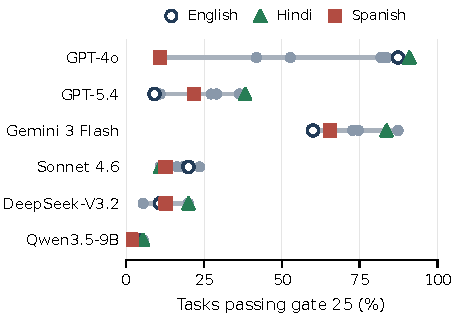
\includegraphics[width=\columnwidth]{figures/fig1_gate_by_language.pdf}
\caption{Pass rates at gate 25 for the same 55 code tasks. Lines span all
eight languages; symbols identify English, Hindi, and Spanish. Other
languages are gray dots. Evaluator short labels follow \S\ref{sec:setup}.}
\Description{Six evaluator rows show language-dependent task pass rates
from zero to one hundred percent.}
\label{fig:gate}\end{figure}

For a fixed evaluator on identical code, the fraction of tasks passing a
satisfaction gate depends heavily on the rubric language: at a gate of 25,
GPT-4o passes 90.9\% in Hindi and 10.9\% in Spanish
(Fig.~\ref{fig:gate}). Sweeping the threshold, the correction cuts
across-language spread by 10.6 to 14.2 percentage points at the tested
gates from 10 to 30, where scores concentrate (Fig.~\ref{fig:sweep}).
The changes are smaller and can worsen spread at higher gates, where fewer
tasks pass. For each evaluator, spread is the maximum minus minimum pass
rate across languages; we report its mean over evaluators.

The direction of the shift differs by evaluator. Comparing the English default
against the mean of the seven localized conditions at gate 25, GPT-4o becomes
stricter when the rubric is localized ($-27.9$ percentage points, 95\% CI
$[-37.7,-18.2]$), while Gemini 3 Flash Preview and GPT-5.4 become
more lenient
($+13.9$ $[+7.0,+21.3]$ and $+15.6$ $[+9.4,+22.3]$). The remaining three
evaluators show contrasts whose intervals include zero. Localizing an
evaluation harness can tighten or loosen the same gate, with the direction
depending on the evaluator. A single language adjustment
cannot remove shifts that differ in sign across evaluators.

A shift shared by all evaluators survives double centering. Its estimated
range is 8.6 points across the eight languages, from Hindi $+5.3$ to Spanish
$-3.3$. It can be centered, but human labels are needed to judge whether
that improves accuracy.


\subsection{Comparison with simpler corrections}

\begin{figure}[t]\centering
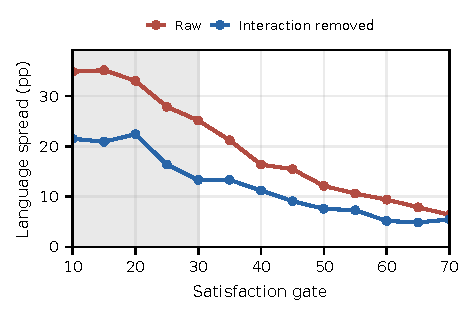
\includegraphics[width=\columnwidth]{figures/fig3_gate_sweep.pdf}
\caption{Mean pass-rate spread across languages as the gate changes.
The shaded range marks gates 10--30. Curves use the saved score panel.}
\Description{Two lines show raw and interaction-corrected language spread
over quality gates from ten to seventy.}
\label{fig:sweep}\end{figure}

The gate endpoint can change under any score transformation.
Table~\ref{tab:base} compares the interaction correction with centering each
language by its overall mean. The interaction correction gives the lowest spread at
each shown gate. In the full panel, gate-25 spread falls from 27.9 to 16.4
percentage points. When we fit on bootstrap samples and evaluate on omitted
tasks, the mean reduction is 8.7 percentage points (95\% percentile interval
$[3.8,14.0]$; 998 of 1{,}000 replicates are positive). This is evidence of
more consistent gates, not more accurate judgments.

\begin{table}[t]\centering\small
\setlength{\tabcolsep}{4pt}\renewcommand{\arraystretch}{1.05}
\caption{Mean language spread in gate pass rates (percentage points) on the
full panel. Bold marks the lowest spread at each gate.}
\label{tab:base}
\begin{tabular*}{\columnwidth}{@{\extracolsep{\fill}}lrrr@{}}
\toprule
\textbf{Correction} & \textbf{Gate 10} & \textbf{Gate 25} & \textbf{Gate 50}\\
\midrule
None (raw)            & 34.8 & 27.9 & 12.1\\
Per-language centering & 39.4 & 28.5 & 12.7\\
CBC ($\hat\beta$) & \textbf{21.5} & \textbf{16.4} & \textbf{7.6}\\
\bottomrule
\end{tabular*}\end{table}

\subsection{Robustness}
\label{sec:robust}

\begin{table*}[t]\centering\small
\caption{Evaluator behavior and leave-one-evaluator-out sensitivity.
Mean score and zero rate use each evaluator's 440 task-level cells.
Interaction magnitudes are score points. Bold identifies GPT-4o's effect
and Qwen3.5-9B's zero-score concentration, not evaluator quality.}
\label{tab:panel}
\begin{tabular*}{\textwidth}{@{\extracolsep{\fill}}lrrrrr@{}}
\toprule
 & \multicolumn{3}{c}{\textbf{Full panel}} & \multicolumn{2}{c}{\textbf{After removing this evaluator}}\\
\cmidrule(lr){2-4}\cmidrule(lr){5-6}
\textbf{Evaluator} & \textbf{Mean score} & \textbf{Zero cells (\%)} & \textbf{Own} $\max|\hat\beta|$ & \textbf{Reversing pairs} & \textbf{Panel} $\max|\hat\beta|$\\
\midrule
Gemini 3 Flash Preview & 42.9 &  2.7 &  9.3 & 6/10 & 20.1\\
GPT-4o   & 33.2 &  6.1 & \textbf{20.6} & \textbf{3/10} & \textbf{8.0}\\
GPT-5.4  & 16.8 & 22.7 &  8.4 & 4/10 & 19.2\\
Claude Sonnet 4.6 & 15.4 & 23.4 &  7.4 & 4/10 & 19.7\\
DeepSeek-V3.2 & 12.2 & 33.0 &  5.7 & 4/10 & 19.7\\
Qwen3.5-9B &  3.6 & \textbf{82.0} &  4.8 & 7/10 & 20.2\\
\bottomrule
\end{tabular*}
\end{table*}

No task drives the effect: leaving out each task in turn moves
$\max|\hat\beta|$ within $[20.2,20.9]$, and no single task moves it by more
than 0.4 points. Table~\ref{tab:panel} shows that removing GPT-4o
reduces reversals from 7/15 to 3/10
pairs and the largest interaction from 20.6 to 8.0 points. Removing any
other evaluator leaves the largest interaction at 19.2 points or more.
The largest effect therefore depends on GPT-4o, though smaller effects
remain. Qwen3.5-9B is a separate concern: it awards zero on 82.0\% of cells and
is close to a constant function, so we also check the panel without it.
Of 52{,}560 requirement judgments, 4.6\% lack a parseable tag or are empty, and
2{,}301 of those 2{,}410 cases are empty Qwen3.5-9B responses: 62\% of its Spanish
requirements and 67\% of its Swahili ones. The released parser scores those
empty strings unsatisfied. Excluding Qwen3.5-9B, the noncompliance rate is 0.12\%,
and GPT-4o's Spanish missing-tag rate is 0.5\%, so missing tags do not
explain the 20.6-point cell.

Because four of the seven reversals involve GPT-4o, we repeat the analysis
without it. Among the five remaining evaluators, the largest interaction is
Gemini 3 Flash Preview in Arabic at $+8.0$ points (95\% CI $[6.3, 9.9]$), and gate spread still
falls from 27.6 to 21.5 points at a gate of 10 and from 17.5 to 13.8 at 25. The
largest interaction is roughly 39\% of its full-panel size. The largest instance depends on
GPT-4o, but an interaction remains in the reduced panel.

Because both the requirement text and the judge instructions are localized,
$\hat\beta$ still mixes judge behavior with specification-translation quality.
A control that keeps requirement text in English and localizes only the
instructions was previously run at 20-task, two-language, one-evaluator scale
\citep{mahmood2026multilingualpromptlocalizationagentasajudge} and found a
large Hindi/Arabic asymmetry under that partial localization. We do not
extend that control to the eight-language, six-evaluator panel here;
$\hat\beta$ should therefore be read as a mixture of judge behavior and
specification-translation quality, which is a limitation of this measurement
rather than a result we claim to have separated.

An additive model on $[0,100]$ can strain linearity at the floor. Recovering
$\hat\beta$ after an arcsin-square-root transform of the satisfaction
proportion agrees with the linear matrix (Spearman $0.97$; no sign flips among
cells with $|\hat\beta|\ge 1$), and the gate-25 spread reduction remains
11.5 points when corrected angles are clipped to $[0,\pi/2]$ before mapping
back to scores. A percentile-rank transform agrees similarly (Spearman $0.95$).
A logit link does not: it flips five of those cells and widens gate spread,
because Qwen3.5-9B's pile-up at zero is mapped to large logit residuals. We keep the
linear correction for the gate endpoint; the logit sensitivity check shows
that conclusions need not survive every transformation.

Double centering removes the variation that cross-language consistency
measures penalize. A higher consistency score therefore cannot show that the
removed term was error. The next section tests repeat-run variation;
\S\ref{sec:anchor} explains why the available human labels cannot support
the planned requirement-level accuracy test with the saved judgments.

%=====================================================================
\section{Replication}
\label{sec:repl}

The released panel holds one judgment per (evaluator, language, framework,
task) cell. It therefore cannot separate repeat-call variation from a
stable language effect. We measure that variation with new calls.

We reran a stratified subset chosen before any call was made: 10
tasks spread across the requirement-count distribution, all eight languages,
all six evaluators, three repeats, and the MetaGPT arm only (1{,}440 calls).
The judge stack, temperature ($0$), top-$p$ ($0.9$), and parser are those of
the original panel. The manifest seed is recorded and is not sent to the
provider. The decision rule was fixed before the reruns: retain the magnitude
claim only if the test--retest standard deviation $s$, averaged over tasks,
languages, and evaluators, is below one quarter of the largest interaction
$B$. Otherwise the claim is qualified or withdrawn as specified in the
analysis script.

The 1{,}440 calls completed. We compute a sample standard deviation across
the three repeats for each task--language--evaluator cell, then average
those standard deviations. Mean test--retest sd is $s=4.08$ points against
$B=20.61$, a ratio of $0.20$, so the prespecified rule passes. The largest
mean sd for one language-by-evaluator cell is 10.9 points; individual tasks
can be noisier. This is a 10-task MetaGPT slice, not a repeat of the full
55-task, three-framework panel. Across languages, mean cell sd ranges
from 3.09 points in English to 5.06 in Spanish; this slice cannot
establish a language-resource trend.

%=====================================================================
\section{Is the Removed Term Error?}
\label{sec:anchor}

The interaction is larger than mean repeat-call variation in the sampled
slice. The language-conditioned term could still encode real
differences in how well a judge reads code when prompted in a given language.
Separating error from competence needs a reference outside the panel. DevAI
ships expert satisfaction labels for the evaluated agents
\citep{zhuge2024agentjudge}; the local export contains 1{,}098 judgments
across the 55 tasks and three agents. The human base rate is 36.5\%
satisfied, so an always-unsatisfied classifier scores 63.5\%
and raw accuracy is misleading. A future human-label test should use
balanced accuracy and Matthews correlation against that baseline, with task
resampling that retains requirements and framework judgments together.
Improvement would support treating the interaction
as error; degradation would suggest it carries useful signal.

Matching a human satisfaction base rate does not establish requirement-level
correctness. A future test should compare paired requirement decisions,
not only aggregate positive rates. The benchmark requirements and human
labels are supplied in English, so results should also be reported with
and without English.

This submission does not run that requirement-level test. The export audit finds five
human-label requirements but four evaluator requirements for task
52\texttt{\_Devin\_AI\_Trains\_an\_AI} in each agent workspace, and the saved
judgments contain binary verdicts without a continuous requirement-level score
from which a corrected verdict can be computed. We therefore report no pooled
balanced-accuracy difference: doing so would require silently reindexing a
requirement or inventing the missing score. The blocked-test audit is included
with the analysis records. A comparison of task scores with aggregated human
satisfaction would address a coarser target and remains untested.

The M-RewardBench panel includes public gold preferences. A previous
analysis reported that panel-mean agreement increased from 68.7\% to
76.6\% after CBC. Rechecking its 700 sampled item-language margins
shows that this increase is a numerical tie artifact: 55 apparent
decision changes have zero raw margin but tiny positive floating-point
corrected margins. Three other margins differ slightly because their
cells are incomplete, without changing their decisions. With a common
absolute-margin tie tolerance of $10^{-9}$, panel-mean agreement is 68.7\% both before and
after CBC. Proposition~\ref{prop:identify} explains why that mean is
invariant on a complete panel. We retract the earlier accuracy gain
and make no human-accuracy claim for CBC.

%=====================================================================
\section*{Limitations}

The test--retest (\S\ref{sec:repl}) is a 10-task MetaGPT slice, not a rerun of
the full 55-task, three-framework panel; a few individual tasks have
three-repeat sds far above the pooled 4.1-point mean. The largest effect
depends on GPT-4o. The external preference panel covers only two
AlpacaEval subsets, with 35 missing margins; the complete-panel
identification result is not exact for this available-case analysis.
Because we do not rerun the instruction-only
control on this panel,
$\hat\beta$ mixes judge behavior with specification-translation quality, which
plausibly varies across the eight languages. The prior two-language ablation
cannot estimate the two sources in this panel. The human-label anchor is blocked by a
requirement-schema mismatch and by binary-only saved judgments; this is not
evidence for a null effect, and corrected scores should not be treated as
ground truth. The interaction correction leaves the language shift shared by
all judges in place. That shift can be centered without labels, but labels
are needed to decide whether doing so improves accuracy.
Finally, the evidence is 55 tasks from one code-evaluation family and six
evaluator routes; the additive model is unbounded while
scores lie in $[0,100]$, which strains the linear approximation near zero.
An arcsin-square-root transform leaves the recovered interaction and the
gate-25 reduction intact; a logit link does not, because of the pile-up at
zero, so the linear correction should not be read as uniquely privileged at
the floor. A deployment should refit and monitor the interaction when
judge versions change; this single panel cannot measure temporal drift.

%=====================================================================
\section*{Conclusion}

The same code can receive different scores and gate decisions when the
judging inputs are localized. The fixed artifacts make this a property of the
judging setup, although they do not separate judge behavior from translation
quality. The language-by-evaluator interaction changes evaluator severity
and gate outcomes; the largest shift exceeds mean repeat-call variation in
the sampled slice. Double centering estimates that interaction without
labels, and the task-level bound allows dependence among judges within
a task. Removing the interaction improves held-out evaluator-score ordering
consistency on DevAI and a separate preference subset, and makes
individual-evaluator gates more consistent. The panel-mean score remains
unchanged, so the previously reported preference-gold gain was spurious.
The corrected scores have not been shown to be more accurate.

\section*{Reproducibility}
Results in \S\ref{sec:results} were recomputed from the saved score
matrices at the reported precision; rare numerical rank-tie differences
are documented in the artifact. The separate preference score panel and the corrected
human-anchor audit are included with the analysis records. The test--retest in
\S\ref{sec:repl} is the 1{,}440-call MetaGPT rerun; its pre-registered
decision file is shipped with the artifact. Human labels are the public
\texttt{human\_as\_a\_judge} release of the Agent-as-a-Judge repository, MIT
licensed.
The codebase records Python 3.11 and a Poetry lockfile; the DevAI
implementation used here is version 0.1.5. The original panel's hardware and
provider snapshot metadata were not preserved, so those analyses can be
recomputed from the saved matrices but not rerun from the original provider
state. The new reruns include model routes and decoding metadata.
AI-assisted tools were used to edit wording and draft analysis and figure
code. The resulting text, calculations, diagrams, and citations were checked against
the saved records and cited sources. The authors remain responsible for the
methods and claims. Further disclosure and available prompts are provided
with the supplementary material, alongside scripts, score matrices, and
replication records.

\section*{Ethics}
No new human subjects were recruited; the human labels are public. The
correction has not been validated for languages outside the panel.
Because a shared
language shift survives it, corrected rankings should not be treated as ground
truth without an external anchor.
The DevAI release is MIT licensed (MIT License, copyright metauto.ai 2024);
the local implementation is version 0.1.5 as recorded in
\texttt{pyproject.toml}.

\bibliographystyle{ACM-Reference-Format}
\bibliography{references}

\end{document}
